\documentclass[a4paper, DIV = calc]{scrartcl}
\usepackage[
typ={ab},
fach=Informatik,
lerngruppe=SG-J1,
%loesungen=seite,
%lizenz={cc-by-nc-sa-4}
module={Aufgaben},
farbig
]{schule}
%\usepackage[libertinus]{fontsetup}
%\usepackage{tikz}
%\usepackage{ctable}
%
%\usepackage{cochineal}
\usepackage{amsmath}
\usepackage{amssymb}
\usepackage{scrlayer-scrpage}
\ifoot{% TODO: \usepackage{graphicx} required
	
	
\includegraphics[width=0.4\linewidth]{GHSE-Logo}
	
}
%\usepackage{fontspec}
%\setmonofont{Monoki}
\usepackage[ngerman]{babel} 
%\usepackage{polyglossia}
%\setmainlanguage{ngerman}  % -> "Contents"
%\setmainlanguage{german}  % -> "Inhaltsverzeichnis"
%\usepackage[utf8]{inputenc}			% Set encoding
%\usepackage[T1]{fontenc}
\usepackage[default]{fontsetup}

\setmonofont{Ubuntu Mono Regular}%[Scale=0.8]
%\setmonofont{Iosevka}%[Scale=0.8]
%\usepackage{polyglossia}
%\setmainlanguage{ngerman}
\usepackage{shellesc}
\ShellEscape{pythontex \jobname.pytxcode }
%\usepackage{minted}
\usepackage{pythontex}
\usepackage{microtype}	
\usepackage[font=tiny,labelfont=bf]{caption}
\usepackage{float}
%\author{Maximilian Hertenstein}
%\date{\today}
\title{Schere-Stein-Papier-Projekt}


%\usepackage{svg}
%\usepackage{ctable}
\date{}

\newcommand{\expandpyconc}[1]{\expandafter\reallyexpandpyconc\expandafter{#1}}
\newcommand{\reallyexpandpyconc}[1]{\pyconc{exec(compile(open('#1', 'rb').read(), '#1', 'exec'))}}

\newenvironment{pyconcodeblck}[1]
{\newcommand{\snippetfile}{snippet-#1.py}
	\VerbatimEnvironment
	\begin{VerbatimOut}{\snippetfile}}
	{\end{VerbatimOut}
	\expandpyconc{\snippetfile}}

\newcommand{\typesetcode}[1]{\inputpygments{python}{snippet-#1.py}}


\hypersetup{hidelinks}
%\usepackage{ctable}
%\usepackage{svg}
%\KOMAoptions{DIV=25}
%\usepackage[default]{fontsetup}
\begin{document}



\begin{pyconcodeblck}{rps}
# -------------- String-Addition

def greet_player_ask_choice_helper(player_name: str) -> str:
    return "Hey " + player_name + "! Please choose rock, paper or scissors! "


# -------------- String-Addition + Typkonversion


def show_round_number(current_round: int, rounds_to_play: int):
    return "Round " + str(current_round) + " of " + str(rounds_to_play)


def greet_player_ask_name_helper(number: int) -> str:
    return "Hello Player " + str(number) + "! What's your name? "


# ------------- Ausgabe

def print_round_number(current_round: int, rounds_to_play: int) -> None:
    print(show_round_number(current_round, rounds_to_play))


# ------------- Bedingungen

def point_or_points(points: int) -> str:
    if points == 1:
        return "point"
    else:
        return "points"


def show_player_points(name: str, points: int) -> str:
    return name + " has " + str(points) + " " + point_or_points(points)


def compute_round_winner(p1: str, p2: str) -> str:
    if p1 == p2:
        return "Nobody"
    if (
        p1 == "rock"
        and p2 == "scissors"
        or p1 == "paper"
        and p2 == "rock"
        or p1 == "scissors"
        and p2 == "paper"
    ):
        return "1"
    else:
        return "2"


def compute_game_winner(player1_points: int, player2_points: int) -> str:
    if player1_points > player2_points:
        return "1"
    elif player2_points > player1_points:
        return "2"
    else:
        return "Nobody"


def result_to_name(winner: str, player_1_name: str, player_2_name: str) -> str:
    if winner == "1":
        return player_1_name
    if winner == "2":
        return player_2_name
    else:
        return winner


def round_or_game(full_game: bool) -> str:
    if full_game:
        return "game"
    else:
        return "round"

def show_round_or_game_winner(name: str, full_game: bool) -> str:
    return name + " wins this " + round_or_game(full_game) + "!"


def show_winner_with_name_helper(winner: str, player_1_name: str, player_2_name: str, full_game: bool) -> str:
    return show_round_or_game_winner(result_to_name(winner, player_1_name, player_2_name), full_game)

def show_round_winner_with_name(round_winner: str, player_1_name: str, player_2_name: str) -> str:
    return show_winner_with_name_helper(round_winner, player_1_name, player_2_name, False)

def show_game_winner_with_name(player_1_name: str, player_2_name: str, player1_points: int, player2_points: int) -> str:
    return show_winner_with_name_helper(compute_game_winner(player1_points, player2_points), player_1_name, player_2_name, True)


def compute_new_points(round_winner: str, player_number: int, current_points: int) -> int:
    if str(player_number) == round_winner:
        return current_points + 1
    else:
        return current_points

# ----------------------- Ausgabe
def print_round_winner_with_name(round_winner: str, player_1_name: str, player_2_name: str) -> None:
    print(show_round_winner_with_name(
        round_winner, player_1_name, player_2_name))


def print_players_points(
    player1_name: str, player2_name: str, player1_points: int, player2_points: int
) -> None:
    print(show_player_points(player1_name, player1_points))
    print(show_player_points(player2_name, player2_points))


def print_game_winner_with_name(
    player_1_name: str, player_2_name: str, player1_points: int, player2_points: int
) -> None:
    print(show_game_winner_with_name(player_1_name, player_2_name,
            player1_points, player2_points, ))

# ------------- Eingabe


def greet_player_ask_name(number: int) -> str:
    return input(greet_player_ask_name_helper(number))


def greet_player_ask_choice(player_name: str) -> str:
    return input(greet_player_ask_choice_helper(player_name))


def play_one_round(
    current_round: int, rounds_to_play: int, player_1_name: str, player_2_name: str
) -> str:
    print_round_number(current_round, rounds_to_play)
    player1_decision = greet_player_ask_choice(player_1_name)
    player2_decision = greet_player_ask_choice(player_2_name)
    round_winner = compute_round_winner(player1_decision, player2_decision)
    print_round_winner_with_name(round_winner, player_1_name, player_2_name)
    return round_winner

# ----------------------- For-Schleifen


def play_rps_helper(
    rounds_to_play: int, player_1_name: str, player_2_name: str
) -> None:
    player_1_points = 0
    player_2_points = 0
    for current_round in range(1, rounds_to_play + 1):
        winner_of_current_round = play_one_round(
            current_round, rounds_to_play, player_1_name, player_2_name)
        player_1_points = compute_new_points(
            winner_of_current_round, 1, player_1_points)
        player_2_points = compute_new_points(
            winner_of_current_round, 2, player_2_points)
        print_players_points(player_1_name, player_2_name,
                             player_1_points, player_2_points)
    print_game_winner_with_name(player_1_name, player_2_name,
                        player_1_points, player_2_points)


def play_rps() -> None:
    player_1_name = greet_player_ask_name(1)
    player_2_name = greet_player_ask_name(2)
    rounds_to_play = int(input("How many rounds do you want to play? "))
    play_rps_helper(rounds_to_play, player_1_name, player_2_name)



# --------------------------------------------------------------------------
# Improvements


def is_in_interval(number_as_str: str, start: int, end: int) -> bool:
    for i in range(start, end + 1):
        if number_as_str == str(i):
            return True
    return False


def greet_player_ask_correct_choice(name: str) -> str:
    print(greet(name))
    return get_correct_choice()


def get_correct_choice() -> str:
    user_input = input("Please choose rock, paper or scissors! ")
    while not (
        user_input == "scissors" or user_input == "paper" or user_input == "rock"
    ):
        print(user_input + " is not a valid choice!")
        user_input = input("Please choose rock, paper or scissors! ")
    # print(20 * "\n")
    return user_input


def greet(name: str) -> str:
    return "Hey, " + name + "!"


def get_correct_number_of_rounds(start: int, end: int) -> int:
    request_to_user = "Please choose a number between " + \
        str(start) + " and " + str(end) + " "
    user_input = input(request_to_user)
    while not (
        is_in_interval(user_input, start, end)
    ):
        print(user_input + " is not a valid choice!")
        user_input = input(request_to_user)
    # print(20 * "\n")
    return int(user_input)


#play_rps_many_rounds()


\end{pyconcodeblck}




\section{String-Addition}
\begin{aufgabe} \noindent 
Implementiere eine Funktion \pygment{python}{greet_player_ask_choice_helper}, die einen Namen als String übergeben bekommt und einen String zurückgibt, in dem die Person gebeten wird, sich für Schere, Stein oder Papier zu entscheiden.
\begin{pyconsole}
greet_player_ask_choice_helper("Anna")
greet_player_ask_choice_helper("Timo")
\end{pyconsole}
\end{aufgabe}



\section{String-Addition und Typkonversion}

\begin{aufgabe} \noindent 
Implementiere eine Funktion \pygment{python}{show_round_number}, die zwei Integer als Argumente übergeben bekommt. Dabei handelt es sich um die Runde die gerade gespielt wird und die Anzahl der Runden, die insgesamt gespielt werden. Die Funktion gibt einen String zurück, in dem beide Informationen enthalten sind.
\begin{pyconsole}
show_round_number(1, 3)
show_round_number(4, 5)
\end{pyconsole}
\end{aufgabe}


\begin{aufgabe} \noindent 
Implementiere eine Funktion \pygment{python}{greet_player_ask_name_helper}. Dieser Funktion wird die Nummer eines Spielers als Integer übergeben. Sie gibt einen String zurück, indem der Spieler begrüßt und nach seinem Namen gefragt wird.
\begin{pyconsole}
greet_player_ask_name_helper(1)
greet_player_ask_name_helper(2)
\end{pyconsole}
\end{aufgabe}

\section{Ausgabe}

\begin{aufgabe} \noindent 
Implementiere eine Funktion \pygment{python}{print_round_number}. Dieser Funktion werden die aktuelle Rundenzahl und die Anzahl der Runden die insgesamt gespielt werden als Integer übergeben. Sie gibt beide Informationen an der Konsole aus.
\begin{pyconsole}
print_round_number(1, 5)
print_round_number(1, 1)
\end{pyconsole}
\hinweis{Nutze \pygment{python}{show_round_number}}
\end{aufgabe}




\section{Bedingungen}


\begin{aufgabe} \noindent 
Implementiere eine Funktion \pygment{python}{point_or_points}. Dieser Funktion wird eine Punktezahl als Integer übergeben. Sie gibt \pygment{python}{"points"} zurück wenn die Zahl $0$ oder größer als eins ist.  Wenn die Zahl $1$ ist, gibt sie \pygment{python}{"point"} zurück.
\begin{pyconsole}
point_or_points(1)
point_or_points(4)
\end{pyconsole}
\end{aufgabe}

\begin{aufgabe} \noindent 
Implementiere eine Funktion \pygment{python}{show_player_points}. Dieser Funktion wird ein Name als String und eine Punktezahl als Integer übergeben. Sie gibt einen String zurück, in dem steht wie viele Punkte die Person hat.
\begin{pyconsole}
show_player_points("Kevin", 1)
show_player_points("Barbara", 3)
\end{pyconsole}
\hinweis{Nutze \pygment{python}{point_or_points}}
\end{aufgabe}

\begin{aufgabe} \noindent
Implementiere eine Funktion \pygment{python}{compute_round_winner}. Dieser werden die Eingaben der beiden Spieler als Strings übergeben. Sie gibt zurück, wer die Runde gewonnen hat. Die einzigen möglichen Argumente sind \pygment{python}{"rock"}, \pygment{python}{"paper"} und \pygment{python}{"scissors"}. Die einzigen möglichen Rückgabewerte sind \pygment{python}{"1"}, \pygment{python}{"2"} und \pygment{python}{"Nobody"}.

\begin{figure}[H]
	%\centerline{\includesvg[inkscapelatex=false,width=0.5\linewidth]{rock-paper-scissors}}
	\centering	
	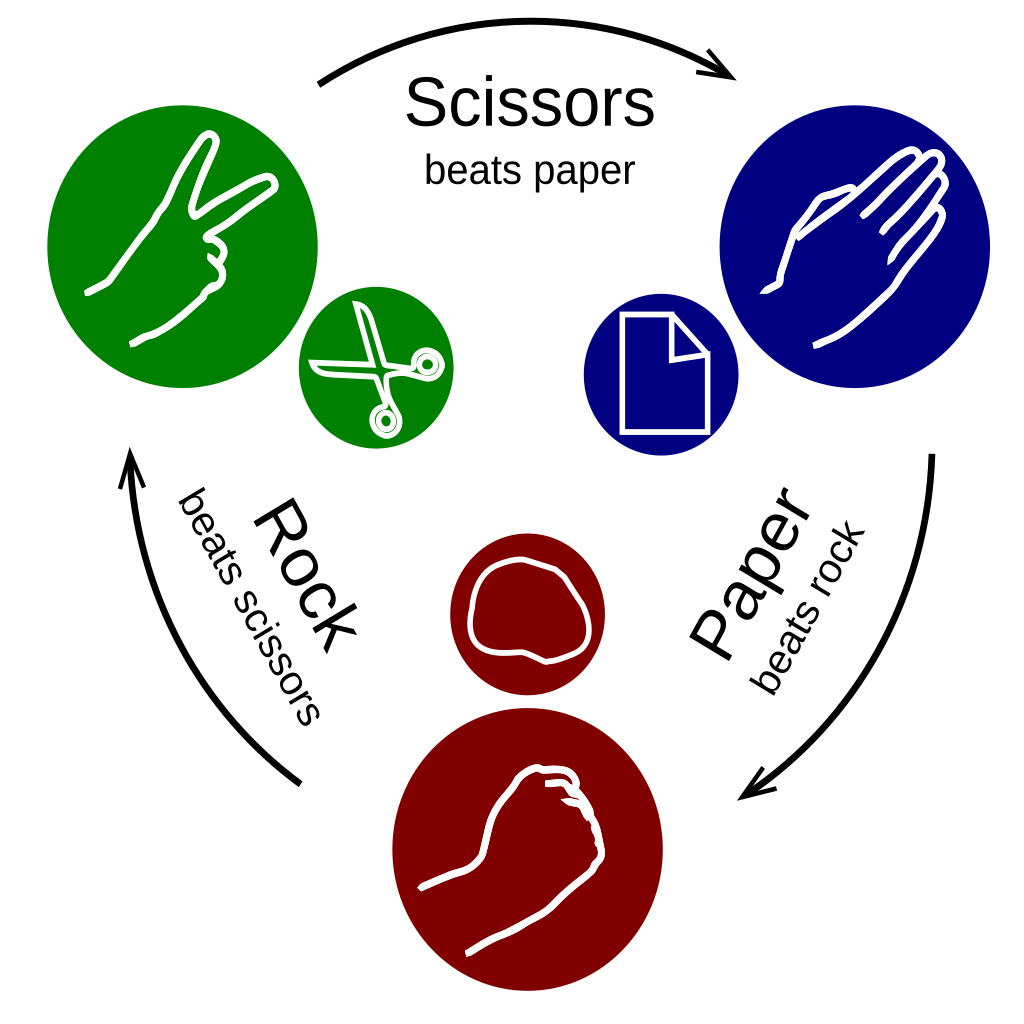
\includegraphics[width=0.5\linewidth]{rock-paper-scissors}
	\tiny \caption{\tiny \url{https://upload.wikimedia.org/wikipedia/commons/6/67/Rock-paper-scissors.svg}}
	%\label{fig: example}
\end{figure}

\begin{pyconsole}
compute_round_winner("rock", "scissors")
compute_round_winner("rock", "paper")
compute_round_winner("rock", "rock")
\end{pyconsole}



\end{aufgabe}


\begin{aufgabe} \noindent 
Implementiere eine Funktion \pygment{python}{compute_game_winner}. Dieser Funktion werden die Punktezahlen der beiden Spieler als Integer übergeben. Sie gibt einen String zurück, in dem steht, wer das gesamte Spiel gewonnen hat. Die einzigen möglichen Rückgabewerte sind \pygment{python}{"1"}, \pygment{python}{"2"} und \pygment{python}{"Nobody"}.
\begin{pyconsole}
compute_game_winner(1, 5)
compute_game_winner(3,  2)
compute_game_winner(3,  3)
\end{pyconsole}

\end{aufgabe}



\begin{aufgabe} \noindent 
Implementiere eine Funktion \pygment{python}{result_to_name}. Dieser Funktion wird der Gewinner einer Runde / eines Spiels und die Namen der Spieler übergeben. Wenn es einen Gewinner gibt, gibt sie seinen Namen zurück Ansonsten wird \pygment{python}{"Nobody"} zurückgegeben. Die einzigen Möglichkeiten für das erste Argument sind \pygment{python}{"1"}, \pygment{python}{"2"} und \pygment{python}{"Nobody"}.
\begin{pyconsole}
result_to_name("1", "John", "Ringo")
result_to_name("2",  "Mick", "Keith")
result_to_name("Nobody",  "Ringo", "George")
\end{pyconsole}

\end{aufgabe}


\begin{aufgabe} \noindent 
Implementiere eine Funktion \pygment{python}{round_or_game}. Dieser wird ein Boolean Übergeben. Wenn dieses \pygment{python}{True} ist, gibt sie \pygment{python}{"game"} zurück. Ansonsten gibt sie \pygment{python}{"round"} zurück.
\begin{pyconsole}
round_or_game(True)
round_or_game(False)
\end{pyconsole}
\end{aufgabe}

\begin{aufgabe}
Implementiere eine Funktion \pygment{python}{show_round_or_game_winner}. Dieser wird ein Name und Boolean übergeben. Wenn \pygment{python}{True} übergeben wird, gibt die Funktion einen String zurück, in dem steht, dass die Person mit diesem Namen das Spiel gewonnen hat. Ansonsten steht in dem String, dass die Person die Runde gewonnen hat.

\begin{pyconsole}
show_round_or_game_winner("John", True)
show_round_or_game_winner("Paul", False)
\end{pyconsole}

\hinweis{Nutze \pygment{python}{round_or_game}}

\end{aufgabe}

\begin{aufgabe}
Implementiere eine Funktion \pygment{python}{show_winner_with_name_helper}. Dieser wird übergeben, wer das Spiel/die Runde gewonnen hat. Die einzigen Möglichkeiten sind  \pygment{python}{"1"}, \pygment{python}{"2"} und \pygment{python}{"Nobody"}. Außerdem werden die Namen der Spieler und ein Boolean übergeben. Wenn dieses \pygment{python}{True} ist soll als String zurückgegeben werden welcher Spieler, das Spiel gewonnen hat. Ansonsten wird zurückgegeben welcher Spieler die Runde gewonnen hat. In dem String werden die übergebenen Namen verwendet.


\begin{pyconsole}
show_winner_with_name_helper("1", "Grace", "Alan", True)
show_winner_with_name_helper("2", "Grace", "Alan", False)
show_winner_with_name_helper("Nobody", "Grace", "Alan", False)
\end{pyconsole}

\hinweis{Nutze \pygment{python}{show_round_or_game_winner} und \pygment{python}{result_to_name}}


\end{aufgabe}

\begin{aufgabe}
eine Funktion \pygment{python}{show_round_winner_with_name}. Dieser wird übergeben wer das Spiel gewonnen hat. Die einzigen Möglichkeiten sind  \pygment{python}{"1"}, \pygment{python}{"2"} und \pygment{python}{"Nobody"}. Außerdem werden die Namen der Spieler übergeben. Die Funktion gibt einen String zurück in dem steht, wer die Runde gewonnen hat. In dem String wird der Name des Spielers verwendet.

\begin{pyconsole}
show_round_winner_with_name("1", "Grace", "Alan")
show_round_winner_with_name("2", "Grace", "Alan")
show_round_winner_with_name("Nobody", "Grace", "Alan")
\end{pyconsole}

\hinweis{Nutze \pygment{python}{show_winner_with_name_helper}}
\end{aufgabe}

\begin{aufgabe}
eine Funktion \pygment{python}{show_game_winner_with_name}. Dieser werden Namen der Spieler als Strings und ihre die Punktezahlen  als Integer  übergeben. Die Funktion gibt einen String zurück in dem steht, wer das Spiel gewonnen hat.

\begin{pyconsole}
show_game_winner_with_name("Grace", "Alan", 1, 2)
show_game_winner_with_name("Grace", "Alan", 5, 0)
show_game_winner_with_name("Grace", "Alan", 1 , 1)
\end{pyconsole}

\hinweis{Nutze \pygment{python}{show_winner_with_name_helper} und \pygment{python}{compute_game_winner}}
\end{aufgabe}

\begin{aufgabe}
Implementiere eine Funktion \pygment{python}{compute_new_points}. Dieser wird der Gewinner der letzten Runde, die Nummer eines Spielers und die Punktzahl des Spielers mit dieser Nummer übergeben. Die einzigen Möglichkeiten für das erste Argument sind  \pygment{python}{"1"}, \pygment{python}{"2"} und \pygment{python}{"Nobody"}.
Die Funktion gibt die neue Punktzahl des Spielers zurück.
\begin{pyconsole}
compute_new_points("1", 1, 3)
compute_new_points("2", 1,  3)
compute_new_points("Nobody", 1, 1)
\end{pyconsole}
\end{aufgabe}


\section{Ausgabe}

\begin{aufgabe}
Schreibe eine Funktion \pygment{python}{print_round_winner_with_name}. Diese funktioniert genau wie \pygment{python}{show_round_winner_with_name}. Sie gibt den Strings aber an der Konsole aus und nicht zurück.

\begin{pyconsole}
print_round_winner_with_name("1", "Grace", "Alan")
print_round_winner_with_name("2", "Grace", "Alan")
print_round_winner_with_name("Nobody", "Grace", "Alan")
\end{pyconsole}
\hinweis{Nutze \pygment{python}{show_round_winner_with_name}}

\end{aufgabe}



\begin{aufgabe} \noindent 
Implementiere eine Funktion \pygment{python}{print_players_points}. Dieser Funktion werden zwei Spielernamen als Strings und deren Punktezahl als Integer übergeben. Sie gibt an der Konsole aus welcher Spieler wie viele Punkte hat.
\begin{pyconsole}
print_players_points("Kevin", "Barbara", 1, 5)
print_players_points("Ali", "Maria", 1, 5)
\end{pyconsole}
\hinweis{Nutze \pygment{python}{show_players_points}}
\end{aufgabe}

\begin{aufgabe} \noindent 
Implementiere eine Funktion \pygment{python}{print_game_winner_with_name}. Dieser Funktion werden zwei Spielernamen als Strings und deren Punktezahl als Integer übergeben. Sie gibt das Endergebniss an der Konsole aus.
\begin{pyconsole}
print_game_winner_with_name("Kevin", "Barbara", 1, 5)
print_game_winner_with_name("Ali", "Maria", 6, 5)
print_game_winner_with_name("Ali", "Maria", 6, 6)
\end{pyconsole}
\hinweis{Nutze \pygment{python}{show_game_winner_with_name}}
\end{aufgabe}

\section{Eingabe}

\begin{aufgabe} \noindent 
Implementiere eine Funktion \pygment{python}{greet_player_ask_name}. Der Funktion wird eine Spielernummer als Integer übergeben. Sie fordert den Spieler dazu auf seinen Namen an der Konsole einzugeben. Der Name wird anschließend zurückgegeben.

\begin{figure}[H]
	%\centerline{\includesvg[inkscapelatex=false,width=0.5\linewidth]{rock-paper-scissors}}
	\centering	
	\includegraphics[width=0.8\linewidth]{greet_player_ask_name}

	%\label{fig: example}
\end{figure}
\hinweis{Nutze \pygment{python}{greet_player_ask_name_helper}}
\end{aufgabe}

\begin{aufgabe}
Schreibe eine Funktion \pygment{python}{ask_rounds}, die fragt wie viele Runden gespielt werden sollen. Diese Eingabe wird als Integer zurückgegeben.

\begin{figure}[H]
	%\centerline{\includesvg[inkscapelatex=false,width=0.5\linewidth]{rock-paper-scissors}}
	\centering	
	\includegraphics[width=0.8\linewidth]{ask_rounds}

	%\label{fig: example}
\end{figure}
\end{aufgabe}

\begin{aufgabe} \noindent 
Implementiere eine Funktion \pygment{python}{greet_player_ask_choice}. Der Funktion wird eine Spielername als String übergeben. Sie fordert die Spielerin dazu auf Schere, Stein oder Papier einzugeben. Die Auswahl wird als String zurückgegeben.

\begin{figure}[H]
	%\centerline{\includesvg[inkscapelatex=false,width=0.5\linewidth]{rock-paper-scissors}}
	\centering	
	\includegraphics[width=0.8\linewidth]{greet_player_ask_choice}

	%\label{fig: example}
\end{figure}
\hinweis{Nutze \pygment{python}{greet_player_ask_choice_helper}}
\end{aufgabe}


%\begin{aufgabe} \noindent 
%Implementiere eine Funktion \pygment{python}{play_rps_helper}. Der Funktion werden die Namen von zwei Spielern übergeben. Sie spricht beide Spielerinnen mit den übergeben Namen an und fordert sie dazu auf Schere, Stein oder Papier einzugeben. Es wird ein String zurückgeben. In diesem String steht, wer gewonnen hat.\\
%\hinweis{Nutze \pygment{python}{greet_player_ask_choice} und \pygment{python}{rps}}
%\begin{figure}[H]
%	%\centerline{\includesvg[inkscapelatex=false,width=0.5\linewidth]{rock-paper-scissors}}
%	\centering	
%	\includegraphics[width=0.8\linewidth]{play_rps_helper}
%
%	%\label{fig: example}
%\end{figure}
%\hinweis{Nutze \pygment{python}{greet_player_ask_choice} und \pygment{python}{rps}!}
%\end{aufgabe}
%
%
%
%\begin{aufgabe} \noindent 
%Implementiere eine Funktion \pygment{python}{play_rps}. Diese Funktion bittet zwei Spieler Schere, Stein oder Papier einzugeben. Anschließend wird ausgegeben, wer gewonnen hat.\\
%
%\begin{figure}[H]
%	%\centerline{\includesvg[inkscapelatex=false,width=0.5\linewidth]{rock-paper-scissors}}
%	\centering	
%	\includegraphics[width=0.8\linewidth]{play_rps}
%
%	%\label{fig: example}
%\end{figure}
%\hinweis{Nutze \pygment{python}{play_rps_helper}!}
%\end{aufgabe}

\begin{aufgabe} \noindent 
Implementiere eine Funktion \pygment{python}{play_one_round}. Dieser Funktion werden die aktuelle Rundenzahl und die Zahl der Runden, die gespielt werden, übergeben. Sie gibt diese beiden Informationen in der Konsole aus. Der Funktion werden auch die Namen der Spieler übergeben. Sie spricht die Spieler mit ihren Namen an und bittet sie Schere, Stein oder Papier einzugeben. Das Ergebnis dieser Runde wird anschließend aus- und gegeben. Hierbei wird der Name des Gewinners genutzt.

Es wird auch zurückgegeben, wer gewonnen hat. Die einzig möglichen Rückgabewerte sind  \pygment{python}{"1"}, \pygment{python}{"2"} und \pygment{python}{"Nobody"}.

\begin{figure}[H]
	%\centerline{\includesvg[inkscapelatex=false,width=0.5\linewidth]{rock-paper-scissors}}
	\centering	
	\includegraphics[width=0.8\linewidth]{play_one_round}

	%\label{fig: example}
\end{figure}

\hinweis{Nutze \pygment{python}{print_round_number}, \pygment{python}{greet_player_ask_choice}, \pygment{python}{compute_round_winner} und \pygment{python}{print_round_winner_with_name}}

\end{aufgabe}


\begin{aufgabe} \noindent 
Implementiere eine Funktion \pygment{python}{play_rps_helper}. Diese Funktion werden die Anzahl der Runden, die gespielt werden und die Namen der Spieler übergeben. Sie spielt das Spiel unter diesen Bedingungen.


Nachdem alle Runden gespielt wurden, wird das Endergebnis ausgegeben.\\ \hinweis{Nutze \pygment{python}{play_one_round}, \pygment{python}{compute_new_points} und  \pygment{python}{print_game_winner_with_name}.}
\begin{figure}[H]
	%\centerline{\includesvg[inkscapelatex=false,width=0.5\linewidth]{rock-paper-scissors}}
	\centering	
	\includegraphics[width=0.8\linewidth]{play_rps_helper}

	%\label{fig: example}
\end{figure}
\end{aufgabe}


\begin{aufgabe} \noindent 
Implementiere eine Funktion \pygment{python}{play_rps}. Diese Funktion fragt zwei Spieler nach ihren Namen. Anschließend fragt sie wie viele Runden gespielt werden sollen. Danach wird das Spiel mit diesen Einstellungen durchgeführt.\\ \hinweis{Nutze \pygment{python}{greet_player_ask_name} und \pygment{python}{play_rps_many_rounds_helper}.}
\begin{figure}[H]
	%\centerline{\includesvg[inkscapelatex=false,width=0.5\linewidth]{rock-paper-scissors}}
	\centering	
	\includegraphics[width=0.8\linewidth]{play_rps}

	%\label{fig: example}
\end{figure}
\end{aufgabe}


\begin{aufgabe}
Nutze das Kontrollzeichen \pygment{python}{"\n"} im Code um bei der Ausgabe Zeilen zu überspringen. 
\end{aufgabe}
\pagebreak
\section{Verbesserungen}

\section{While-Schleifen}
\begin{aufgabe} \noindent
Implementiere eine Funktion \pygment{python}{get_correct_input}, die den Benutzer solange auffordert etwas einzugeben, bis die Eingabe  \pygment{python}{rock},  \pygment{python}{paper} oder  \pygment{python}{scissors} ist. Diese Eingabe wird dann zurückgegeben.
\begin{figure}[H]
	%\centerline{\includesvg[inkscapelatex=false,width=0.5\linewidth]{rock-paper-scissors}}
	\centering	
	\includegraphics[width=\linewidth]{while_input}

\end{figure}

\end{aufgabe}

\begin{aufgabe}
\noindent
Implementiere eine Funktion \pygment{python}{is_in_interval}, die eine Zahl als String und zwei Zahlen als Integer übergeben bekommt. Die Funktion prüft, ob die erste Zahl zwischen den beiden anderen Zahlen liegt. Gehe davon aus, dass das zweite Integer größer ist, als das erste Integer.
\begin{pyconsole}
is_in_interval("4", 1 , 2)
is_in_interval("3", 1 , 3)
is_in_interval("5", 5 , 7)
\end{pyconsole}
\end{aufgabe}



\begin{aufgabe}
\noindent
Implementiere eine Funktion \pygment{python}{get_correct_round_counter}, die zwei Zahlen als Integer übergeben bekommt. Die Funktion fordert die Benutzerin auf eine Rundenzahl zwischen diesen beiden Zahlen einzugeben und fragt solange nach, bis die Eingabe korrekt war.
\end{aufgabe}

\begin{figure}[H]
	%\centerline{\includesvg[inkscapelatex=false,width=0.5\linewidth]{rock-paper-scissors}}
	\centering	
	\includegraphics[width=\linewidth]{get_correct_round_counter}

\end{figure}

\begin{aufgabe}
Bau diese Funktionen in das vollständige Programm ein! 
\end{aufgabe}


%\section{Aufgaben zum Kapitel \enquote{Typen, Werte, Ausdrücke, Operatoren}}
%
%
%\begin{aufgabe} \noindent
%Erkläre die folgenden Begriffe:
%\begin{teilaufgaben}
%\teilaufgabe Operator
%\teilaufgabe Operand
%\teilaufgabe Ausdruck
%\teilaufgabe Typ
%\teilaufgabe Typfehler
%\teilaufgabe Wert
%\teilaufgabe Statement
%\teilaufgabe Befehl
%\end{teilaufgaben}
%\end{aufgabe}
%
%\begin{aufgabe} \noindent
%Beantworte für jeden Ausdruck ob er fehlerfrei ausgewertet werden kann. Bestimme für jeden Ausdruck, der ausgewertet werden kann, den Wert und den Typ.
%\begin{teilaufgaben}
%		\teilaufgabe \pygment{python}{1 + 2 * (1000 - 33)}
%		\teilaufgabe \pygment{python}{"1" + "2" + "3"}
%		\teilaufgabe \pygment{python}{"4" + 5 + "6"}
%\end{teilaufgaben}
%
%\end{aufgabe}
%
%
%\section{Aufgaben zum Kapitel \enquote{Funktionen}}
%
%\begin{aufgabe} \noindent
%	Wie kann der Ausdruck \pygment{python}{7 + 8 + "9"} mit Funktionen zur Typkonversion angepasst werden, damit dass Ergebnis
%	\begin{teilaufgaben}
%		\teilaufgabe \pygment{python}{24} ist?
%		\teilaufgabe \pygment{python}{"789"} ist?
%	\end{teilaufgaben}
%\end{aufgabe}
%
%\section{Aufgaben zum Kapitel \enquote{Skriptmodus}}
%\begin{aufgabe} \noindent
%
%Implementiere ein Skript, das in einer Zeile deinen Vornamen und einer zweiten Zeile deinen Nachnamen ausgibt.
%\end{aufgabe}
%
%\section{Aufgaben zum Kapitel \enquote{Funktionen definieren}}
%
%Implementiere die Lösungen der folgenden Aufgaben in ein Skript mit dem Namen \texttt{functions\_1.py}\\
%
%
%\achtung{Verwende bei jeder Funktion die vollständige und korrekte Typannotation!}\\
%
%
%
%%\begin{aufgabe} \noindent
%%	Implementiere eine Funktion \pygment{python}{good_morning}, die einen Namen als String übergeben bekommt und der Person auf der Konsole \enquote{Guten Morgen!} wünscht.
%%\end{aufgabe}
%
%\begin{aufgabe} \noindent
%Implementiere eine Funktion \pygment{python}{good_morning}, die einen Namen als String übergeben bekommt und der Person auf der Konsole \enquote{Guten Morgen!} wünscht.
%\end{aufgabe}
%
%\begin{pyconsole}
%good_morning("Alan Turing")
%\end{pyconsole}
%
%\begin{aufgabe} \noindent
%\begin{teilaufgaben}
%	\teilaufgabe Implementiere eine Funktion \pygment{python}{hours_to_minutes}, die ein Integer nimmt, das eine Zeit in Stunden angibt und die selbe Zeit in Minuten zurückgibt.
%	\teilaufgabe Implementiere eine Funktion \pygment{python}{days_to_hours}, die ein Integer nimmt, das eine Zeit in Tagen angibt und die selbe Zeit in Stunden zurückgibt.
%	\teilaufgabe Implementiere eine Funktion \pygment{python}{days_to_minutes}, die ein Integer nimmt, das eine Zeit in Tagen angibt und die selbe Zeit in Minuten zurückgibt. Nutze die vorherigen Teilaufgaben!
%\end{teilaufgaben}
%\end{aufgabe}
%
%\begin{pyconsole}
%hours_to_minutes(13)
%days_to_hours(2)
%days_to_minutes(1)
%\end{pyconsole}
%
%
%
%
%
%
%
%
%
%\newpage
%\section{Mehr Aufgaben}
%
%\subsection{Integer}
%
%
%
%
%
%
%\url{https://www.codewars.com/kata/58261acb22be6e2ed800003a/train/python}
%
%
%\url{https://www.codewars.com/kata/55f73be6e12baaa5900000d4/train/python}\\
%
%
%\subsection{Strings}
%
%
%
%
%
%
%\url{https://www.codewars.com/kata/544675c6f971f7399a000e79/train/python}\\
%
%
%
%\url{https://www.codewars.com/kata/5265326f5fda8eb1160004c8/train/python}\\
%
%
%
%\subsection{Booleans}
%
%
%\url{https://www.codewars.com/kata/551b4501ac0447318f0009cd/train/python}\\
%
%
%
%
%
%
%
%
%
%\subsection{Modulo}
%\url{https://www.codewars.com/kata/555086d53eac039a2a000083/train/python}\\
%
%
%
%
%
%
%
%
%
%
%
%
%\subsection{Floats}
%\url{https://www.codewars.com/kata/57a429e253ba3381850000fb/train/python}\\
%
%\section{Bedingungen}
%
%
%
%
%
%
%
%
%
%
%
%
%%\url{https://www.codewars.com/kata/57089707fe2d01529f00024a/train/python}\\
%
%
%
%
%
%
%
%
%
%
%
%
%
%
%%\url{https://www.codewars.com/kata/57e3f79c9cb119374600046b/train/python}\\
%
%
%\section{For-Schleifen}
%
%\subsection{Grundlagen}
%
%
%
%
%\url{https://www.codewars.com/kata/55caef80d691f65cb6000040/train/python}\\
%
%% \url{https://www.codewars.com/kata/528e95af53dcdb40b5000171/train/python}\\
%
%\url{https://www.codewars.com/kata/57241e0f440cd279b5000829/train/python}\\
%
%%\url{https://www.codewars.com/kata/555eded1ad94b00403000071/train/python}\\
%
%
%
%\subsection{Sehr anspruchsvoll}
%
%
%
%
%%\url{https://www.codewars.com/kata/56269eb78ad2e4ced1000013/train/python}\\
%
%
%
%
%%\url{https://www.codewars.com/kata/59a8570b570190d313000037}\\
%
%%\url{}\\
%%\url{}\\
%
%
%
%\section{While-Schleifen}
%
%\subsection{Grundlagen}
%%\url{https://www.codewars.com/kata/534d0a229345375d520006a0/train/python}\\
%
%\url{https://www.codewars.com/kata/57be674b93687de78c0001d9/train/python}\\
%
%% \url{https://www.codewars.com/kata/563b662a59afc2b5120000c6/train/python}\\
%
%
%
%\url{https://www.codewars.com/kata/58941fec8afa3618c9000184/train/python}\\
%
%
%\url{https://www.codewars.com/kata/55f2b110f61eb01779000053/train/python}\\
%
%\subsection{Sehr anspruchsvoll}
%
%\url{https://www.codewars.com/kata/588425ee4e8efb583d000088/train/python}\\
%
%
%\url{https://www.codewars.com/kata/577a6e90d48e51c55e000217/train/python}\\
%
%\url{https://www.codewars.com/kata/5286b2e162056fd0cb000c20/train/python}\\
%
%
%
%\url{https://www.codewars.com/kata/56d46b8fda159582e100001b/train/python}\\
%
%%\url{https://www.codewars.com/kata/57241e0f440cd279b5000829/train/python}\\
%
%\url{https://www.codewars.com/kata/56ba65c6a15703ac7e002075/train/python}\\
%
%
%
%
%
%
%%\url{https://www.codewars.com/kata/5a58d46cfd56cb4e8600009d/train/python}\\
%
%\url{https://www.codewars.com/kata/54c27a33fb7da0db0100040e/train/python}\\
%
%\url{https://www.codewars.com/kata/562f91ff6a8b77dfe900006e/train/python}\\
%
%
%
%\section{Variablen}
%\url{https://www.codewars.com/kata/5612e743cab69fec6d000077/train/python}\\
%
%
%\section{Strings - Iteration}
%\url{https://www.codewars.com/kata/57eae20f5500ad98e50002c5/train/python}\\
%
%\url{https://www.codewars.com/kata/596fba44963025c878000039/train/python}\\
%
%\url{https://www.codewars.com/kata/56b1f01c247c01db92000076/train/python}\\
%
%\url{https://www.codewars.com/kata/56bf3287b5106eb10f000899/train/python}\\
%
%\url{https://www.codewars.com/kata/52f3149496de55aded000410/train/python}\\
%
%%\url{}\\
%\section{Listen}
%
%\url{https://www.codewars.com/kata/52a723508a4d96c6c90005ba/train/python}\\
%
%\url{https://www.codewars.com/kata/57cc975ed542d3148f00015b/train/python}\\
%
%%\url{https://www.codewars.com/kata/511f0fe64ae8683297000001/train/python}\\
%
%%\url{https://www.codewars.com/kata/511f0fe64ae8683297000001/train/python}\\
%
%%\url{https://www.codewars.com/kata/525c1a07bb6dda6944000031/train/python}\\
%
%
%%\url{https://www.codewars.com/kata/57cc975ed542d3148f00015b/train/python}\\
%
%%\url{https://www.codewars.com/kata/5951d30ce99cf2467e000013/train/python}\\
%
%%\url{https://www.codewars.com/kata/57f781872e3d8ca2a000007e/train/python}\\
%
%%\url{https://www.codewars.com/kata/5266876b8f4bf2da9b000362}\\
%%\url{}\\


\end{document}
